\section{Embedding}

CNN 中的卷积就是一种离散卷积,本质上就是利用一个共享参数的过滤器(Kernel)。图数
据和图像数据的差别在于节点邻居个数、次序都是不定的。

生活中很多数据不具备规则的空间结构,称为Non Euclidean data,如,推荐系统、电子交易、分子结构等抽象出来的图谱。流形也是典型的非欧结构。
\begin{itemize}
    \item 1D:社交网络(eg:Facebook,Twitter等)
    \item 2D:生物网络(基因,分子,大脑连接)等
    \item 3D:基础设施网络(eg:能源,交通,互联网,通信等)
\end{itemize}

社交网络非常适合用图数据来表达,社交网络中节点以及节点与节点之间的关系,用户A(有ID信息等)、用户B、帖子都是节点,用户与用户之间的关系是关注,用户与帖子之间的关系可能是发布或者转发。

图的空间结构特征:
\begin{itemize}
    \item  节点特征:每个节点有自己的特征;(体现在点上)
    \item  结构特征:图数据中的每个节点具有结构特征,即节点与节点存在一定的联系。(体现在边上)
\end{itemize}

图卷积的核心思想是利用『边的信息』(Edge)对『节点信息』(Vertex)进行『聚合』(Aggregate)从而生成新的『节点表示』。

图神经网络将深度学习方法延伸到非欧几里得的图数据上,大大提高了图数据应用的精度。

\begin{myExample}
    对于一个简单的电商的图,其包含卖家,商品和用户三个关键节点,其中,商品节点关联商品类别节点,用户节点关联注册 IP 节点和 注册地址节点。当用户在购买商品时,用户节点和商品节点就会关联交易节点,同时,交易节点也会关联用户下单时所对应的 IP 节点以及收获地址节点,对应的图结构如下图所示。
    \begin{figure}[htb!]
        \centering
        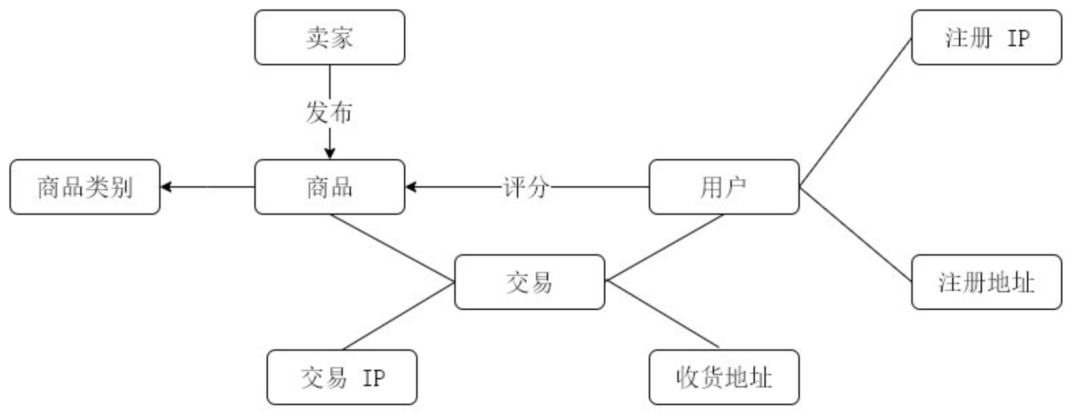
\includegraphics[scale = 0.35]{goods.png}
        \caption{卖家 \& 商品 \& 用户关系图 }
    \end{figure}
    \begin{itemize}
        \item  节点分类—反欺诈:图中每个节点都拥有自己的特征信息,通过该特征信息,我们可以构建一个风控系统,如果交易节点所关联的用户 IP 和收货地址与用户注册 IP 和注册地址不匹配,那么系统将有可能认为该用户存在欺诈风险。
        \item  边结构预测—商品推荐:图中每个节点都具有结构信息。如果用户频繁购买某种类别商品或对某种类别商品评分较高,那么系统就可以认定该用户对该类商品比较感兴趣,
    \end{itemize}
\end{myExample}
